\documentclass[twoside,12pt]{article}
\usepackage{amsmath,amsfonts,amsthm,fullpage,amssymb}
\usepackage{algorithm}
\usepackage{algorithmic}
\usepackage{graphicx}
\usepackage{tcolorbox}


\begin{document}

\title{ISYE 6740, Fall 2020, Homework 3\\{\small 100 points + 15 bonus points}}
\author{Prof. Yao Xie}
\date{}
\maketitle

\subsection*{1. Density estimation: Psychological experiments. (45 points)}

We will use this data to study whether or not the two brain regions are likely to be independent of each other and considering different types of political view \textbf{For this question; you can use the proper package for histogram and KDE; no need to write your own.} The data set \textsf{n90pol.csv} contains information on 90 university students who participated in a psychological experiment designed to look for relationships between the size of different regions of the brain and political views. The variables \textsf{amygdala} and \textsf{acc} indicate the volume of two particular brain regions known to be involved in emotions and decision-making, the amygdala and the anterior cingulate cortex; more exactly, these are residuals from the predicted volume, after adjusting for height, sex, and similar body-type variables. The variable \textsf{orientation} gives the students' locations on a five-point scale from 1 (very conservative) to 5 (very liberal).  Note that in the dataset, we only have observations for orientation from 2 to 5. 
  
 \begin{enumerate}
 
 
 \item[(a)] (10 points) Form the 1-dimensional histogram and KDE to estimate the distributions of \textsf{amygdala} and \textsf{acc}, respectively. For this question, you can ignore the variable \textsf{orientation}.
 \begin{tcolorbox}
 \textbf{Solution:} \\
 \begin{center}
  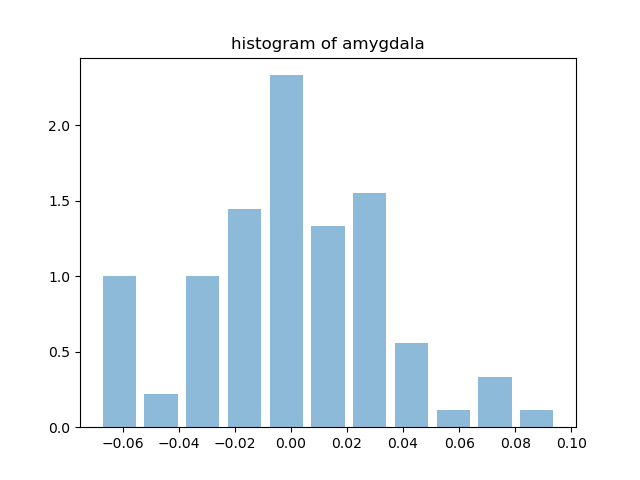
\includegraphics[width=.48\textwidth]{hist_amy.png}
  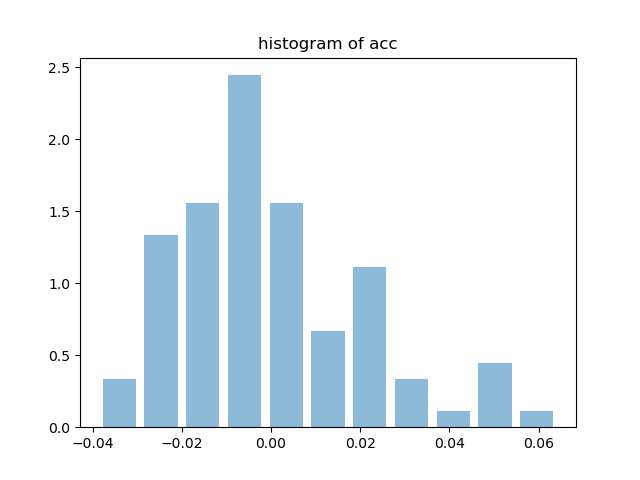
\includegraphics[width=.48\textwidth]{hist_acc.png}
  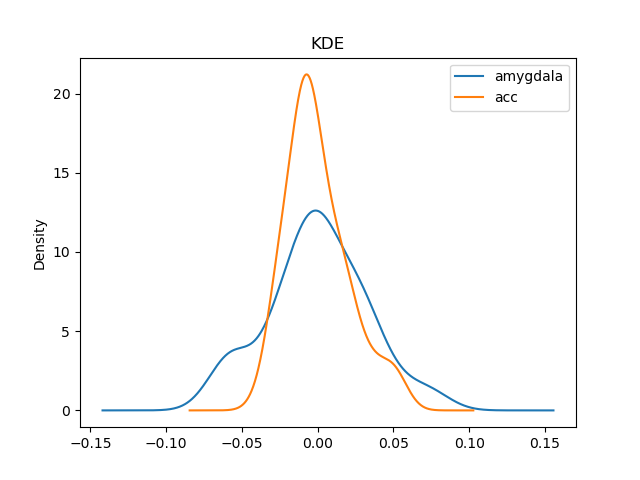
\includegraphics[width=.8\textwidth]{kde.png}
  \end{center}
 \end{tcolorbox}
 
 
 \item[(b)] (10 points) Form 2-dimensional histogram for the pairs of variables (\textsf{amygdala}, \textsf{acc}). Decide on a suitable number of bins so you can see the shape of the distribution clearly. Also use kernel-density-estimation (KDE) to estimate the 2-dimensional density function of (\textsf{amygdala}, \textsf{acc}). Use a simple multi-dimensional Gaussian kernel, for \[x = \begin{bmatrix}x_1\\x_2\end{bmatrix}\in \mathbb R^2,\] where $x_1$ and $x_2$ are the two dimensions respectively \[K(x) = \frac{1}{2\pi} e^{-\frac{(x_1)^2 + (x_2)^2}{2}}.\] Recall in this case, the kernel density estimator (KDE) for a density is given by
 \[
 p(x) = \frac 1 m \sum_{i=1}^m \frac 1 h
 K\left(
 \frac{x^i - x}{h}
 \right),
 \]
where $x^i$ are two-dimensional vectors, $h >0$ is the kernel bandwidth. Set an appropriate $h$ so you can see the shape of the distribution clearly. Plot the contour plot (like the ones in slides) for your estimated density. For this question, you can ignore the variable \textsf{orientation}. 
\begin{tcolorbox}
 \textbf{Solution:} For the Histogram, I used $14$ bins. For the KDE, I tried several values of bandwidth, including $\{0.05, 0.025, 0.015, 0.01, 0.0075, 0.005\}$. As we can see from the following results, when the bandwidth is large, the density function is very smooth and simple. However, when we take smaller bandwidth values, the density function begins to focus more on the details. So we need to choose a proper bandwidth, in this case it was $0.015$, to see the shape of the distribution clearly.  
 \end{tcolorbox}
 \begin{center}
 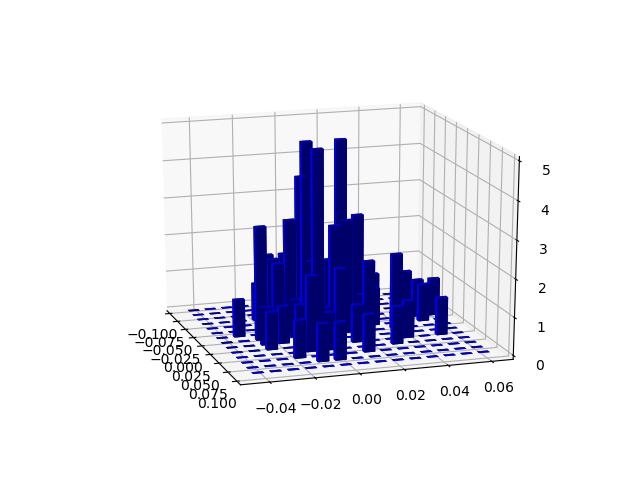
\includegraphics[width=.6\textwidth]{2d_hist.png}\\
% \end{center}
% \end{tcolorbox}
% \newpage
% \begin{tcolorbox}
% \begin{center}
 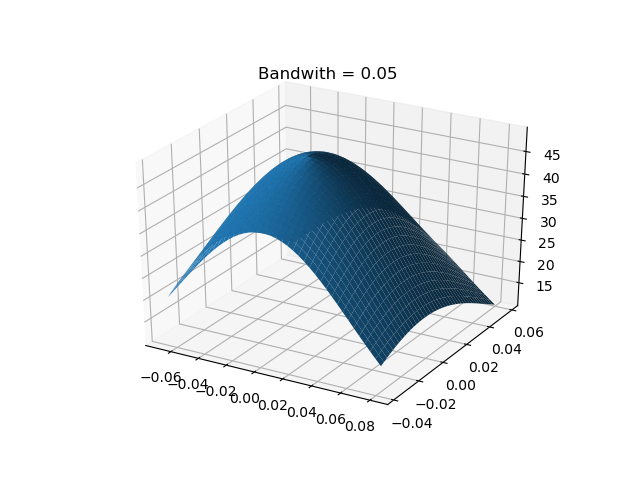
\includegraphics[width=.3\textwidth]{kde1.png}
 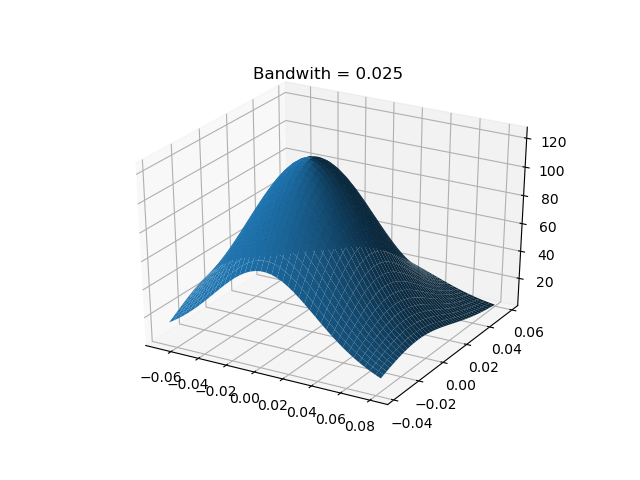
\includegraphics[width=.3\textwidth]{kde2.png}
 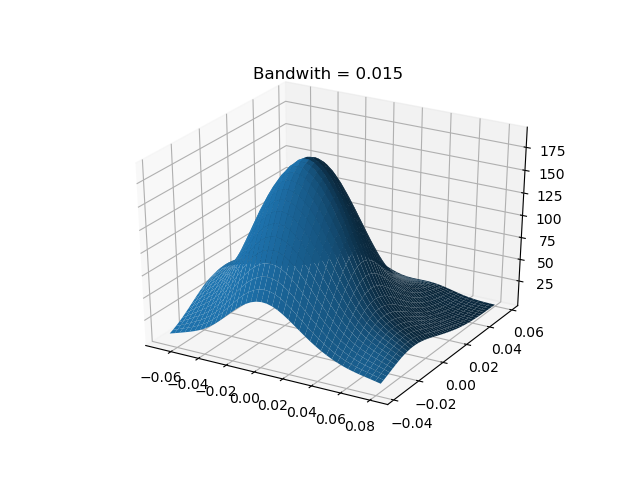
\includegraphics[width=.3\textwidth]{kde3.png}
 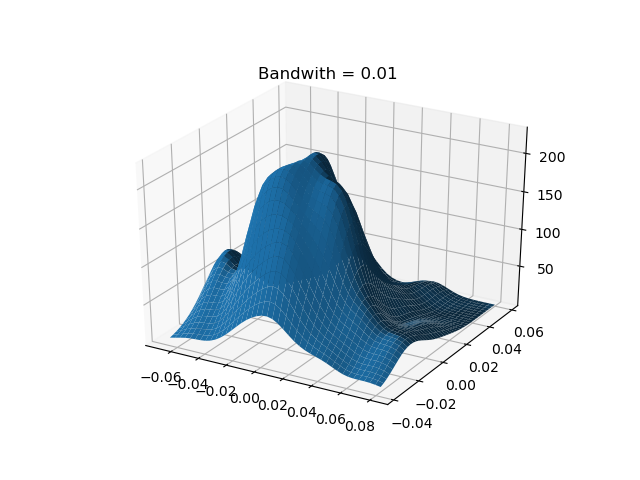
\includegraphics[width=.3\textwidth]{kde4.png}
 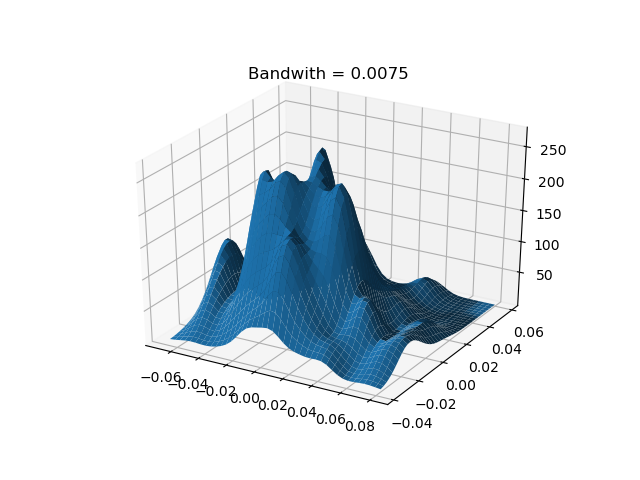
\includegraphics[width=.3\textwidth]{kde5.png}
 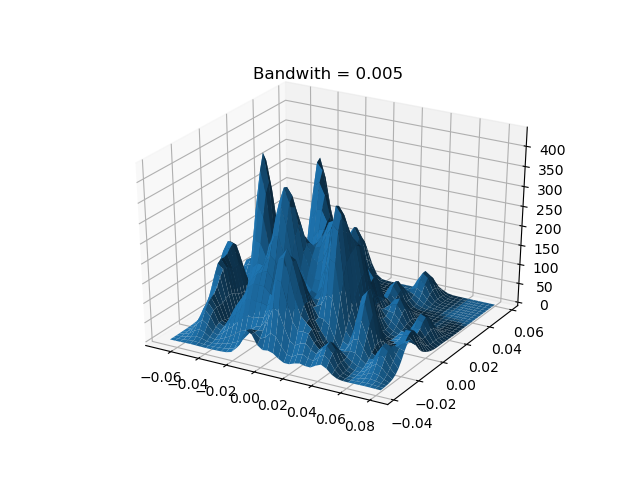
\includegraphics[width=.3\textwidth]{kde6.png}
 \end{center}
 %\end{tcolorbox}
 

 \item[(c)] (10 points) Using (a) and (b), using KDE estimators, verify whether or not  the variables \textsf{amygdala} and \textsf{acc} are independent? You can tell this by checking do we approximately have $p( \textsf{amygdala},  \textsf{acc}) = p( \textsf{amygdala}) p(\textsf{acc})$? To verify this, please show three plots: the map for $p( \textsf{amygdala},  \textsf{acc})$, the map for $p( \textsf{amygdala}) p(\textsf{acc})$ and the error map $|p( \textsf{amygdala},  \textsf{acc}) - p( \textsf{amygdala}) p(\textsf{acc})|$. Comment on your results and whether this helps us to find out whether the two parts of brains (for emotions and decision-making) functions independently or they are related. 
\begin{tcolorbox}
 \textbf{Solution:} In this part, I used two methods to generate the kernel density function, Scipy stats and Sklearn KernelDensity. Scipy stats determines the bandwidth automatically so the bandwidths for the three kernel density functions might be different, while Sklearn Kernel Density allows us to manually assign the bandwidth so that I set all the bandwidth to be $0.01$.\\
 
 \noindent The figures in the first row are obtained by Scipy and figures in the second row are obtained by using Sklearn. I think the results show that the two variables 
 \textsf{amygdala} and \textsf{acc} are independent. Even though their difference is not precisely zero, but the magnitudes are much smaller compared to the original magnitudes.
 \begin{center}
 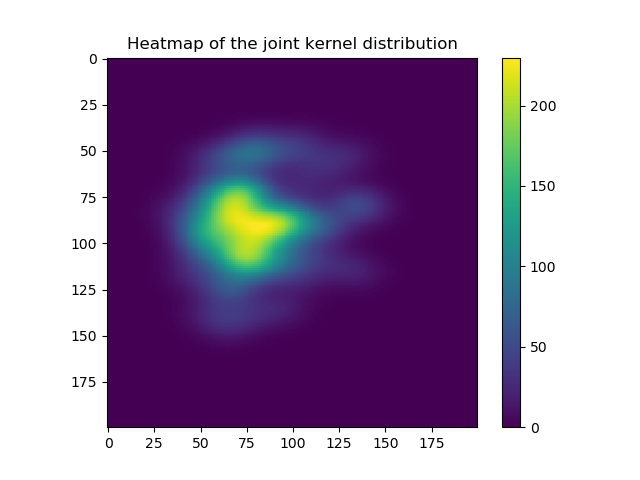
\includegraphics[width=.3\textwidth]{joint.png}
 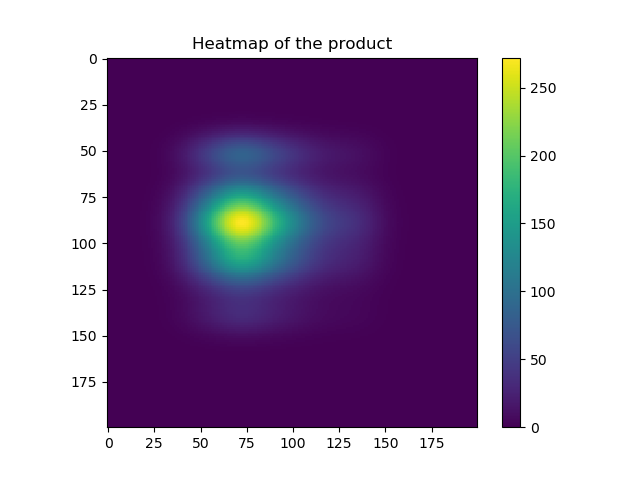
\includegraphics[width=.3\textwidth]{product.png}
 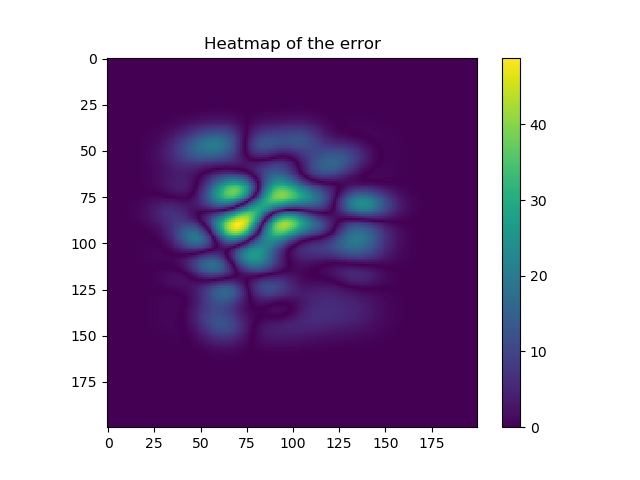
\includegraphics[width=.3\textwidth]{difference.png}
 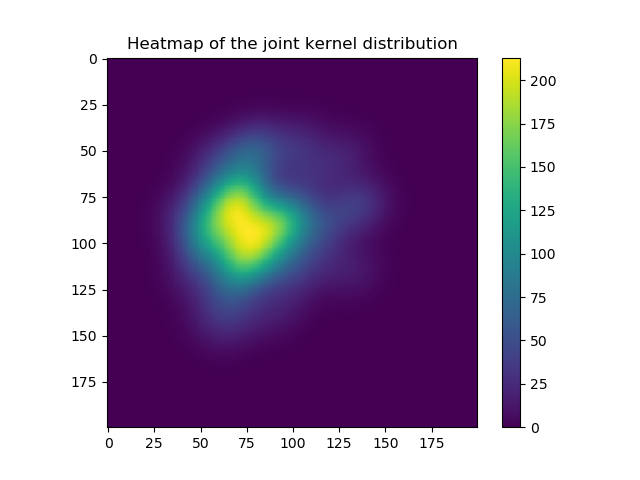
\includegraphics[width=.3\textwidth]{scipy_joint.png}
 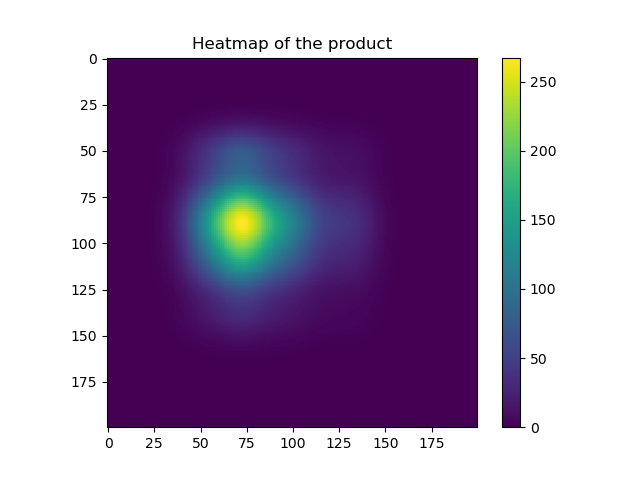
\includegraphics[width=.3\textwidth]{scipy_product.png}
 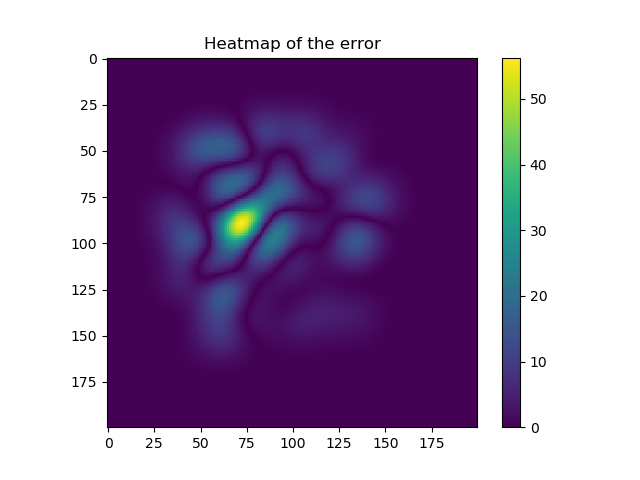
\includegraphics[width=.3\textwidth]{scipy_difference.png}
 \end{center}
 \end{tcolorbox}
 
 
 \item[(d)] (5 points) Now we will consider the variable \textsf{orientation}. We will estimate the conditional distribution of the volume of the \textsf{amygdala}, conditioning on political \textsf{orientation}: $p(\textsf{amygdala}|\textsf{orientation}=c)$, $c = 2, \ldots, 5$. Do the same for the volume of the \textsf{acc}: Plot $p(\textsf{acc}|\textsf{orientation}=c)$, $c = 2, \ldots, 5$. You will use KDE to achieve the goal. (Note that the conditional distribution can be understood as fitting a distribution for the data with the same (fixed) $\textsf{orientation}$. Thus there should be 4 one-dimensional distribution functions to show for this question.) 
\begin{tcolorbox}
 \textbf{Solution:}
 \begin{center}
 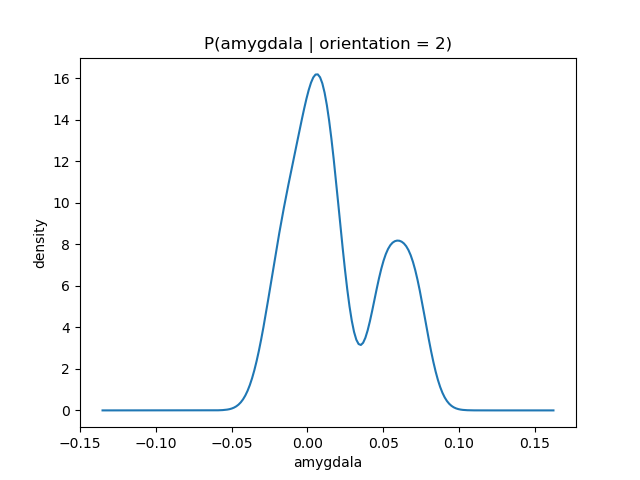
\includegraphics[width=.23\textwidth]{amygdala2.png}
 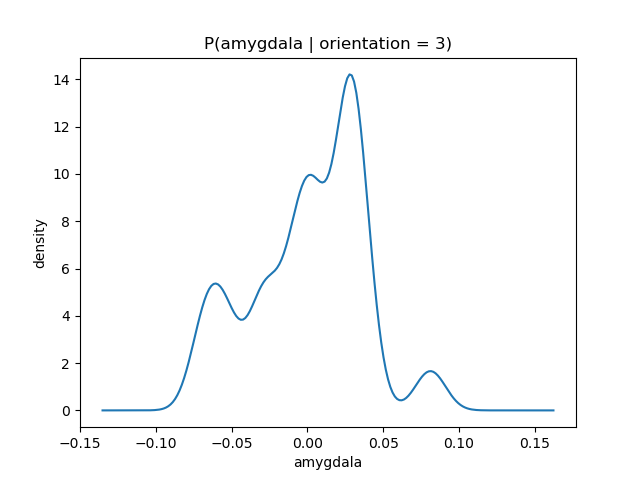
\includegraphics[width=.23\textwidth]{amygdala3.png}
 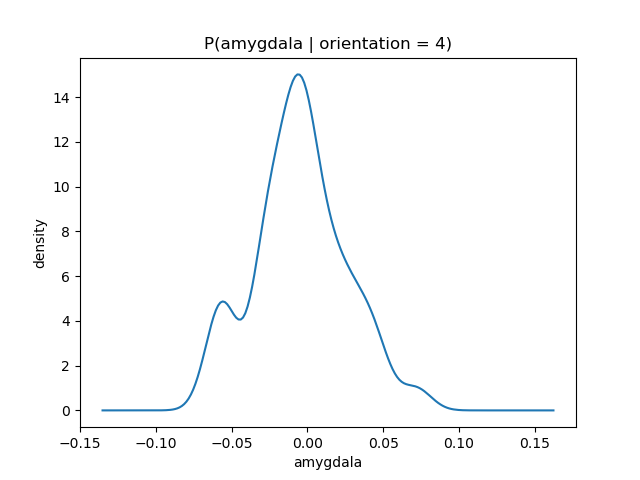
\includegraphics[width=.23\textwidth]{amygdala4.png}
 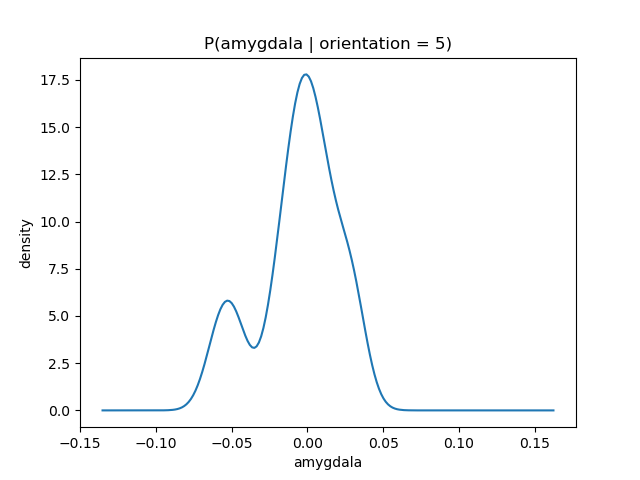
\includegraphics[width=.23\textwidth]{amygdala5.png}
 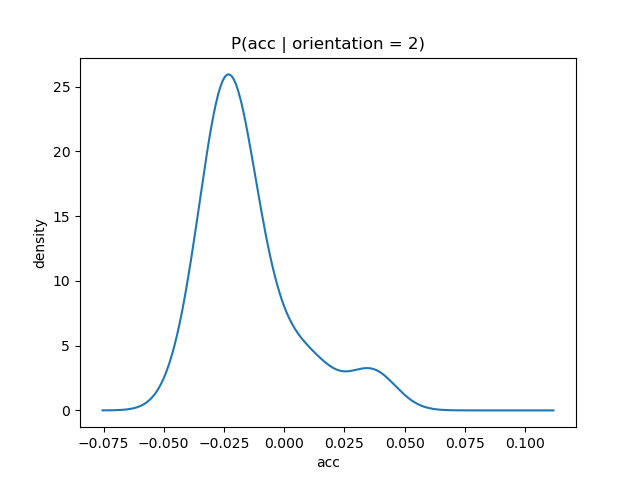
\includegraphics[width=.23\textwidth]{acc2.png}
 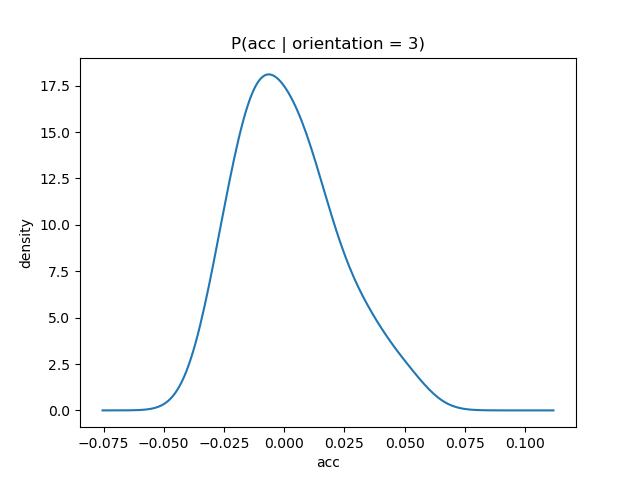
\includegraphics[width=.23\textwidth]{acc3.png}
 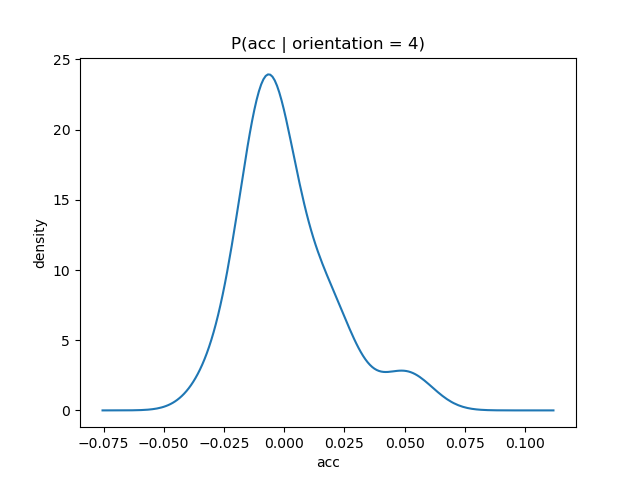
\includegraphics[width=.23\textwidth]{acc4.png}
 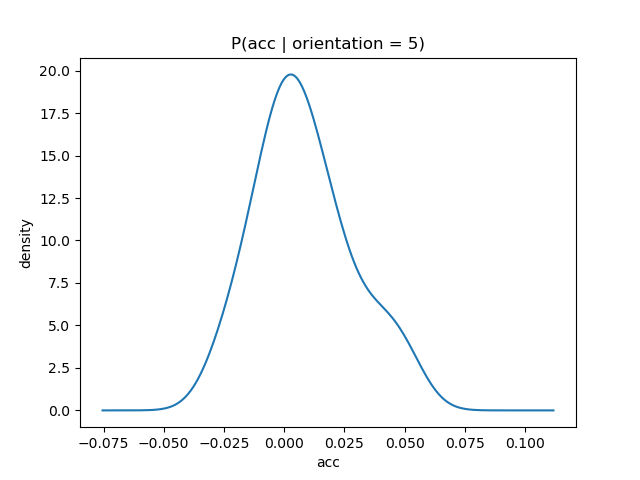
\includegraphics[width=.23\textwidth]{acc5.png}
 \end{center}
 \end{tcolorbox}
  
 \item[(e)] (5 points) Again we will consider the variable \textsf{orientation}. We will estimate the conditional {\it joint} distribution of the volume of the \textsf{amygdala} and \textsf{acc}, conditioning on  a function of political \textsf{orientation}: $p(\textsf{amygdala}, \textsf{acc}|\textsf{orientation}=c)$, $c = 2, \ldots, 5$.  You will use two-dimensional KDE to achieve the goal. 
 \begin{tcolorbox}
 \textbf{Solution:}
 \begin{center}
 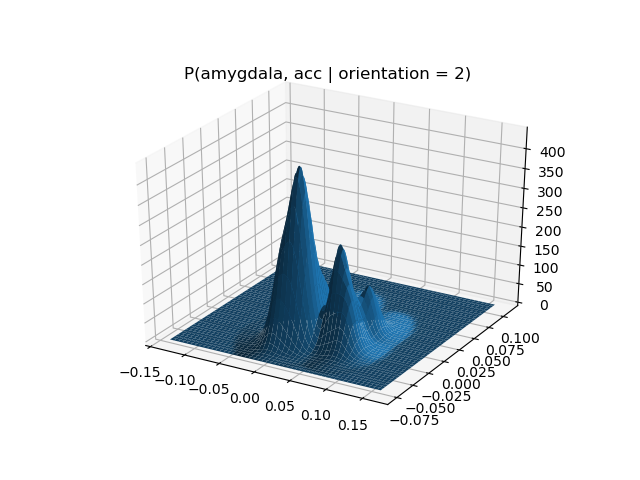
\includegraphics[width=.23\textwidth]{joint_surface2.png}
 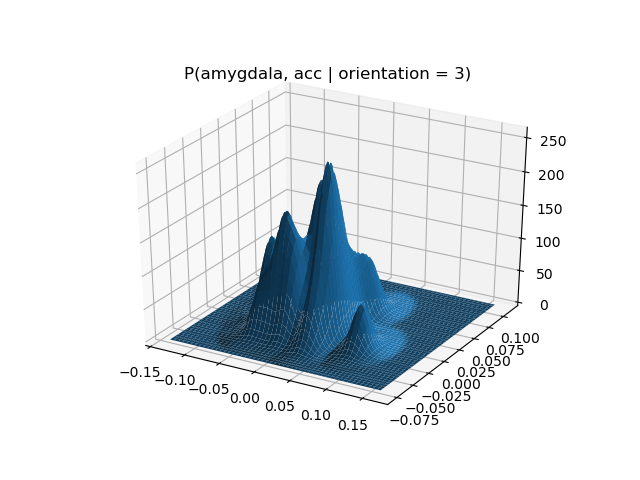
\includegraphics[width=.23\textwidth]{joint_surface3.png}
 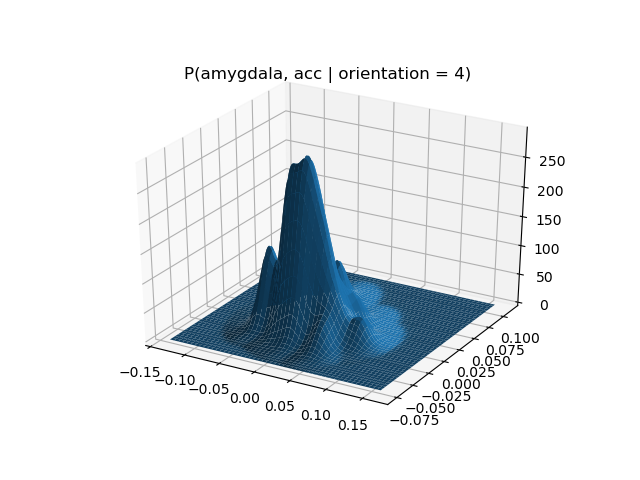
\includegraphics[width=.23\textwidth]{joint_surface4.png}
 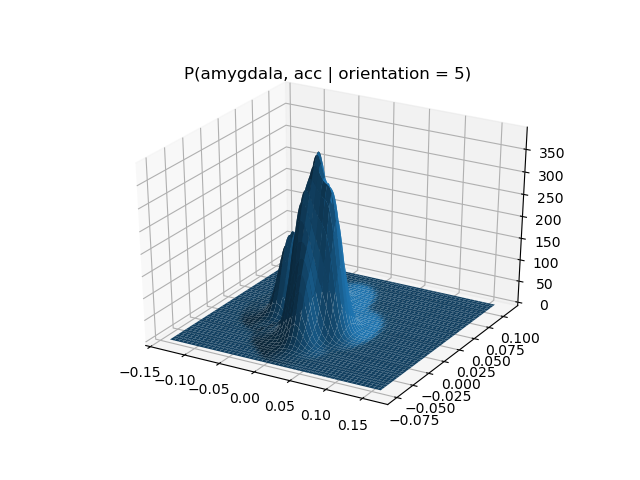
\includegraphics[width=.23\textwidth]{joint_surface5.png}
 \end{center}
 \end{tcolorbox}
 
 \item[(f)] (5 points) Using (d) and (e), evaluate whether or not the two variables are likely to be conditionally independent. To verify this, please show three plots: the map for \[p( \textsf{amygdala},  \textsf{acc}|\textsf{orientation}=c),\] the map for \[p( \textsf{amygdala}|\textsf{orientation}=c) p(\textsf{acc}|\textsf{orientation}=c)\] and the error map 
 \[|p( \textsf{amygdala},  \textsf{acc}|\textsf{orientation}=c) - p( \textsf{amygdala}|\textsf{orientation}=c) p(\textsf{acc}|\textsf{orientation}=c)|,\] 
 $c = 2, \ldots, 5.$ Comment on your results and whether this helps us to find out whether the two parts of brains (for emotions and decision-making) functions independently or they are related, conditionally on the political orientation (i.e., considering different types of personality). 
 \begin{tcolorbox}
 \textbf{Solution:} Since the errors in the two pictures in the middle are less than the errors on the two sides, the results showed that for people who's political views are not extreme, i.e. \textsf{orientation} =  3 or 4, their two parts of brains functions more independently than those with extreme political views, i.e. \textsf{orientation} = 2 or 5.
 \begin{center}
 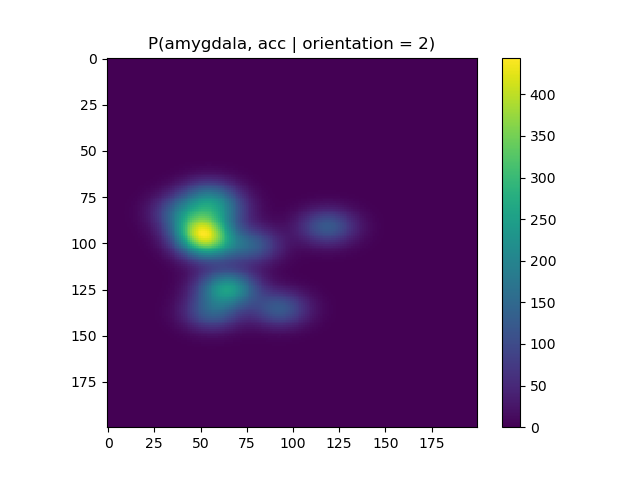
\includegraphics[width=.23\textwidth]{joint2.png}
 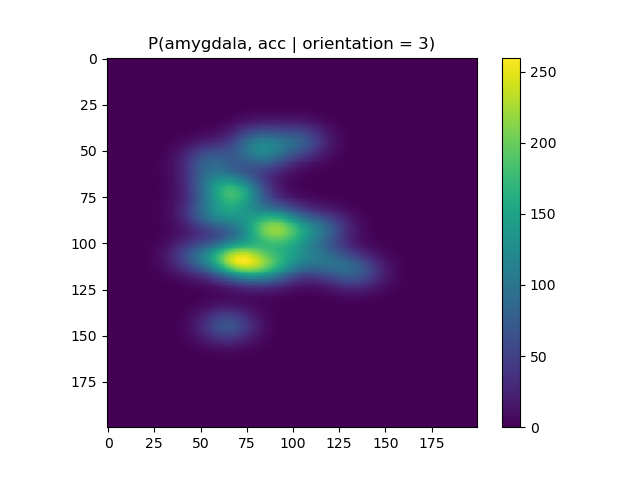
\includegraphics[width=.23\textwidth]{joint3.png}
 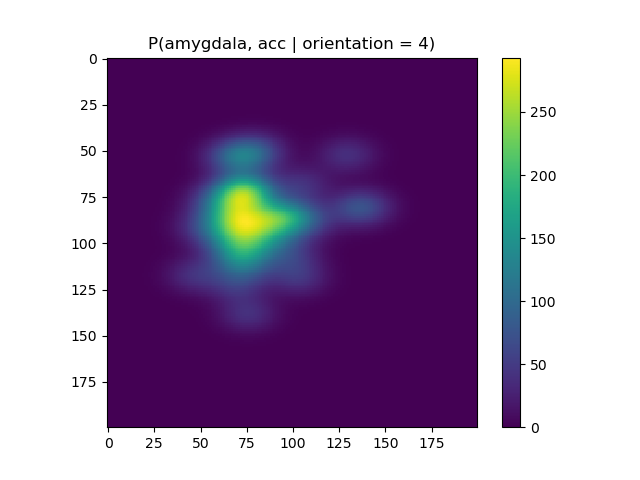
\includegraphics[width=.23\textwidth]{joint4.png}
 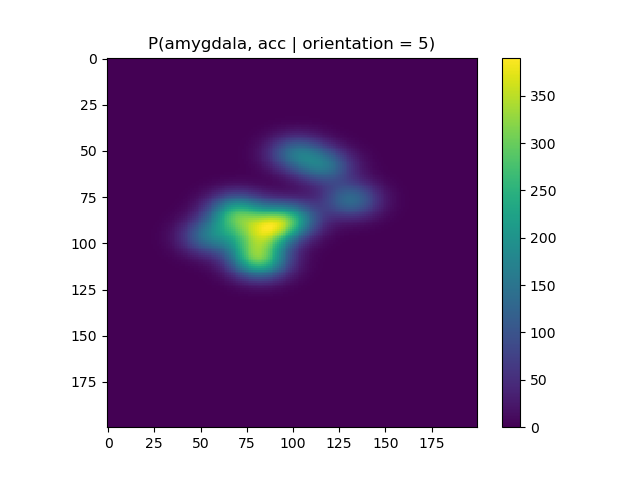
\includegraphics[width=.23\textwidth]{joint5.png}
 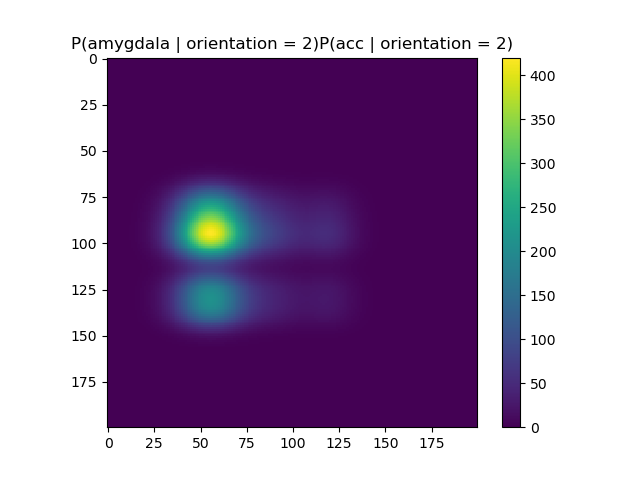
\includegraphics[width=.23\textwidth]{product2.png}
 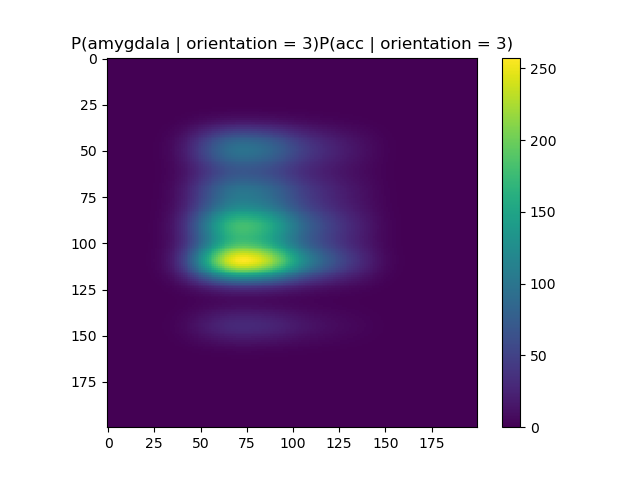
\includegraphics[width=.23\textwidth]{product3.png}
 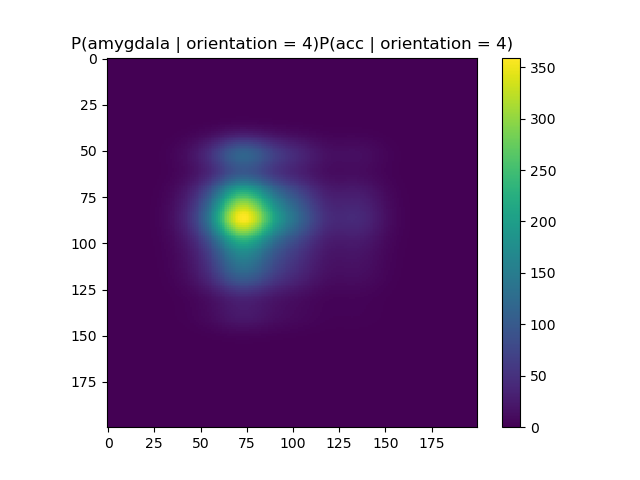
\includegraphics[width=.23\textwidth]{product4.png}
 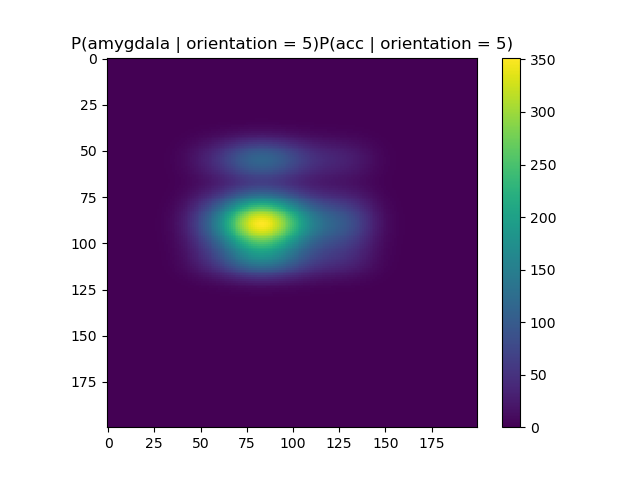
\includegraphics[width=.23\textwidth]{product5.png}
 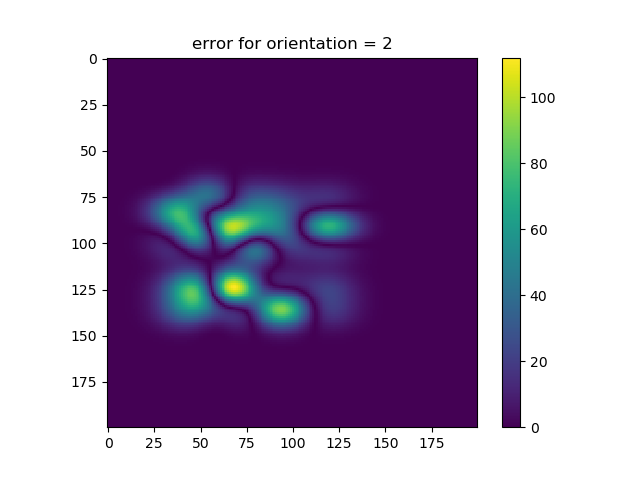
\includegraphics[width=.23\textwidth]{error2.png}
 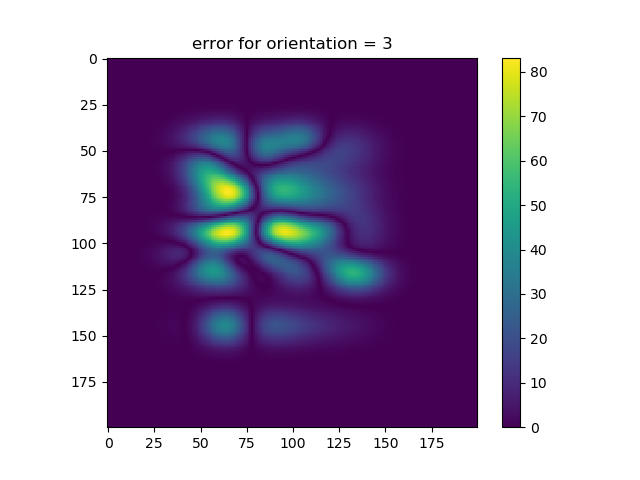
\includegraphics[width=.23\textwidth]{error3.png}
 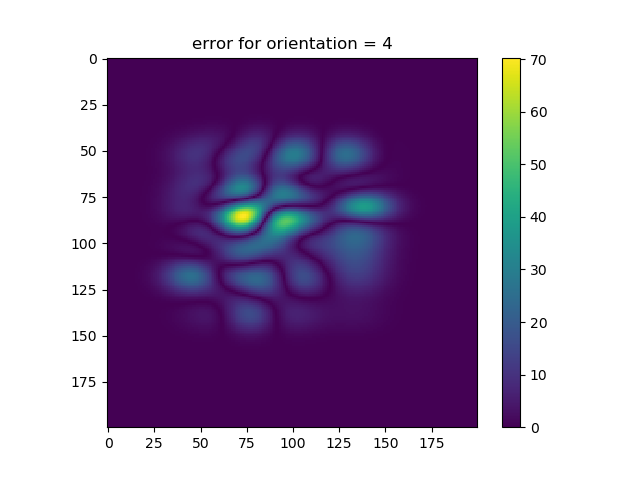
\includegraphics[width=.23\textwidth]{error4.png}
 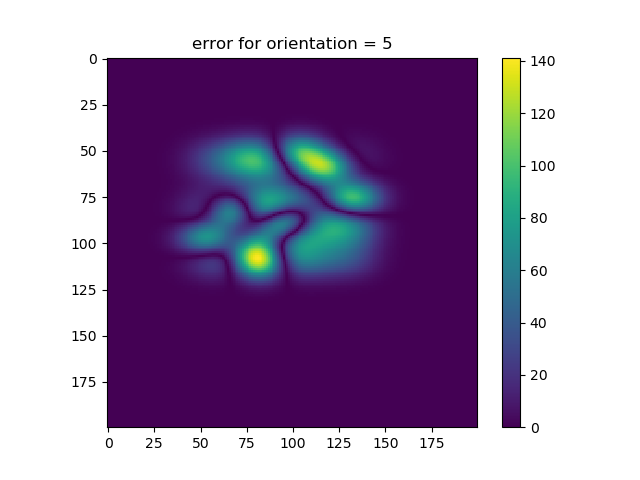
\includegraphics[width=.23\textwidth]{error5.png}
 \end{center}
 \end{tcolorbox} 
 \end{enumerate}




\subsection*{2. Implementing EM for MNIST dataset, with PCA for dimensionality reduction. (55 points)}

Implement the EM algorithm for fitting a Gaussian mixture model for the MNIST dataset. We reduce the dataset to be only two cases, of digits ``2'' and ``6'' only. Thus, you will fit GMM with $C = 2$. Use the data file \textsf{data.mat} or \textsf{data.dat}. True label of the data are also provided in \textsf{label.mat} and \textsf{label.dat}


The matrix \textsf{images} is of size 784-by-1990, i.e., there are totally 1990 images, and each column of the matrix corresponds to one image of size 28-by-28 pixels (the image is vectorized; the original image can be recovered by map the vector into a matrix). 

First use PCA to reduce the dimensionality of the data before applying to EM. We will put all ``6'' and ``2'' digits together, to project the original data into 5-dimensional vectors. Now implement EM algorithm for the projected data (with 5-dimensions). 
\begin{enumerate}

\item[(a)] (5 points) Select from data one raw image of ``2'' and ``6'' and visualize them, respectively. 
\begin{tcolorbox}
 \textbf{Solution:}\\
 \begin{center}
  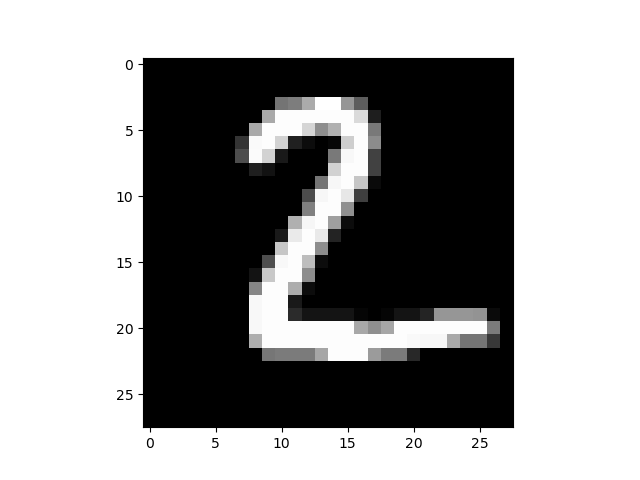
\includegraphics[width=.48\textwidth]{Figure_2.png}
  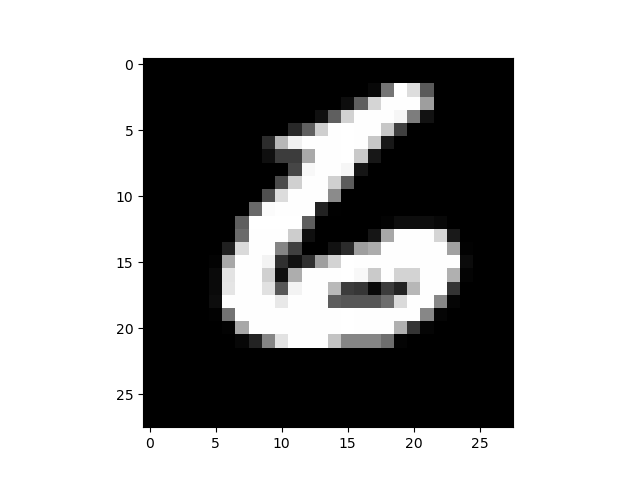
\includegraphics[width=.48\textwidth]{Figure_6.png}
  \end{center}
 \end{tcolorbox}
 
\item[(b)] (10 points) Write down detailed expression of the E-step and M-step in the EM algorithm (hint: when computing $\tau_k^i$, you can drop the $(2\pi)^{n/2}$ factor from the numerator and denominator expression, since it will be canceled out; this can help avoid some numerical issues in computation).
\begin{tcolorbox}
 \textbf{Solution:}\\
 - \textbf{Expectation step (E-step):} Applying the Bayes Formula and the pdf of multivariable Gaussian distribution, we can update $\tau_k^i$ given current $(\pi_k, \mu_k, \Sigma_k)$ in this way:
 $$\tau_k^i  = \frac{\pi_k\mathcal{N}(x^i|\mu_k,\Sigma_k)}{\sum_{k'=1}^K\pi_{k'}\mathcal{N}(x^i|\mu_{k'},\Sigma_{k'})} = \frac{\frac{\pi_k}{|\Sigma_k|^{1/2}}  \exp (-\frac{1}{2} (x^i - \mu_k)^T\Sigma_k^{-1}(x^i-\mu_k))}{\sum_{k'=1}^K \frac{\pi_{k'}}{|\Sigma_{k'}|^{1/2}}\exp (-\frac{1}{2} (x^i - \mu_{k'})^T\Sigma_{k'}^{-1}(x^i-\mu_{k'}))}, $$
for $k = 1, 2, ..., K$, $i = 1, 2, ..., m$.\\

- \textbf{Maximization step (M-step):} Maximizing a lower bound function of log-likelihood function with the constraint $\sum_k \pi_k = 1$ using Lagrange multiplier, we can  update $(\pi_k, \mu_k, \Sigma_k)$ given current $\tau_k^i$ in this way:
$$\pi_k = \frac{\sum_i \tau_k^i}{m}, \quad\quad \mu_k = \frac{\sum_i \tau_k^i x^i}{\sum_i \tau_k^i},$$
$$\Sigma_k = \frac{\sum_i \tau_k^i (x^i - \mu_k)(x^i - \mu_k)^T}{\sum_i \tau_k^i},$$
for $k = 1, 2, ..., K$, $i = 1, 2, ..., m$.
 \end{tcolorbox}
 
\item[(c)] (15 points) Implement EM algorithm yourself. Use the following initialization
\begin{itemize}
\item initialization for mean: random Gaussian vector with zero mean
\item initialization for covariance: generate two Gaussian random matrix of size $n$-by-$n$: $S_1$ and $S_2$, and initialize the covariance matrix for the two components are $\Sigma_1 = S_1 S_1^T + I_n$, and  $\Sigma_2 = S_2 S_2^T + I_n$, where $I_n$ is an identity matrix of size $n$-by-$n$. 
\end{itemize}
Plot the log-likelihood function versus the number of iterations to show your algorithm is converging.
\begin{tcolorbox}
\textbf{Solution:} The EM algorithm stopped after 11 iterations. 
 \begin{center}
  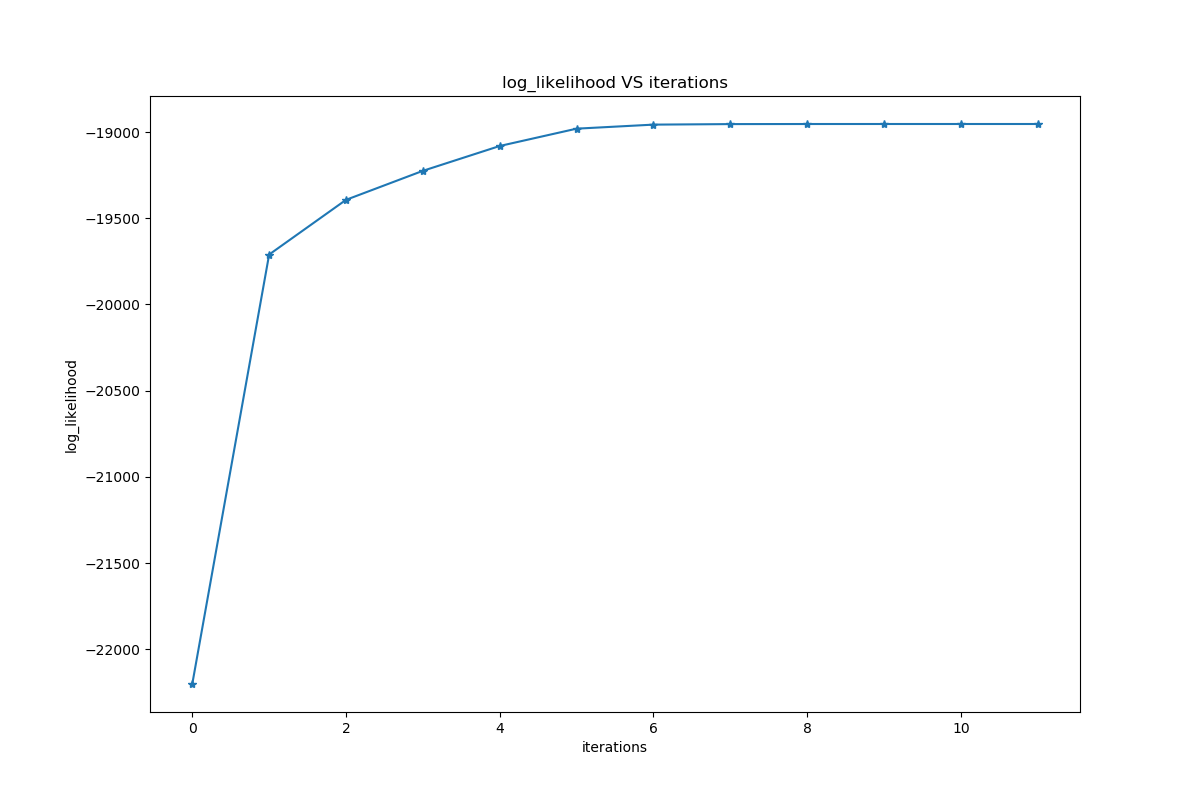
\includegraphics[width=.8\textwidth]{log_likelihood.png}
    \end{center}
 \end{tcolorbox}

\item[(d)] (15 points points) Report, the fitted GMM model when EM has terminated in your algorithms as follows. Make sure to report the weights for each component, and the mean of each component (you can reformat the vector to make them into 28-by-28 matrices and show images). Ideally, you should be able to see these means corresponds to ``average'' images.  Report the two 784-by-784 covariance matrices by visualize their intensities. 

\begin{tcolorbox}
 \textbf{Solution:} The GMM with EM is so powerful! The weight for the cluster of ``6'' is $0.51$ and the weight for the cluster ``2'' is $0.49$. \\
 \begin{center}
  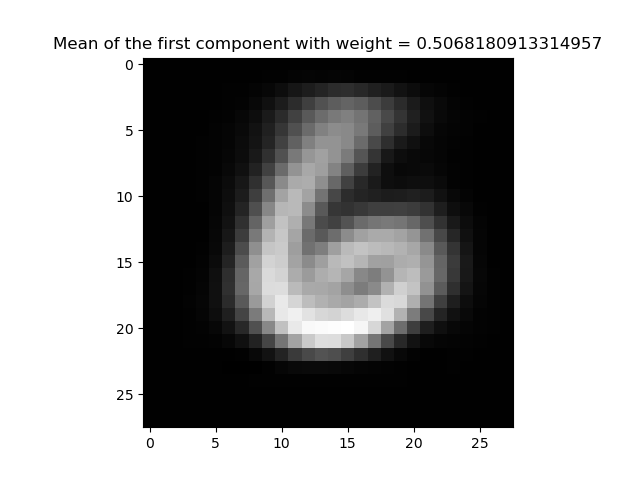
\includegraphics[width=.48\textwidth]{mean1.png}
  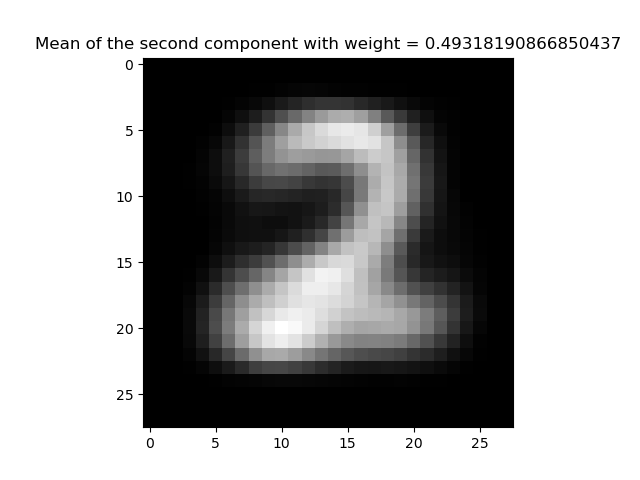
\includegraphics[width=.48\textwidth]{mean2.png}
  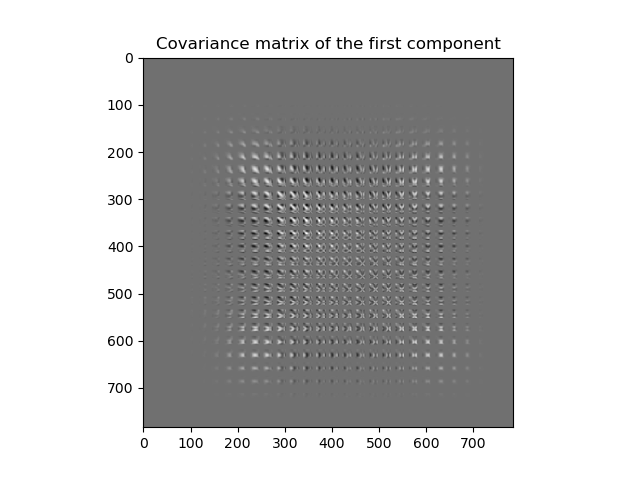
\includegraphics[width=.48\textwidth]{cov1.png}
  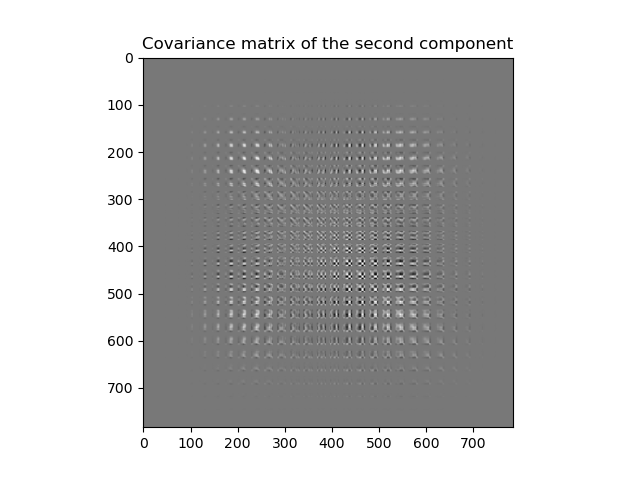
\includegraphics[width=.48\textwidth]{cov2.png}
  \end{center}
 \end{tcolorbox}

\item[(e)] (10 points) Use the $\tau_{k}^i$ to infer the labels of the images, and compare with the true labels. Report the mis-classification rate for digits ``2'' and ``6'' respectively. Perform $K$-means clustering with $K=2$ (you may call a package or use the code from your previous homework). Find out the  mis-classification rate for digits ``2'' and ``6'' respectively, and compare with GMM. Which one achieves the better performance?
\begin{tcolorbox}
\textbf{Solution:} For image $i$, if $\tau_0^i > \tau_1^i$, we predict it to have label ``2'', otherwise ``6''. The mis-classification rate for digits ``2''  is $5.81\%$ and the mis-classification rate for digits ``6''  is $0.73\%$. \\

For Kmeans, I used my own code. The mis-classification rate for digits ``2''  is $7.36\%$ and the mis-classification rate for digits ``6''  is $4.49\%$.\\

Apparently, GMM did a better job! It achieved a lower mis-classification rate for both clusters. 
\end{tcolorbox}

\end{enumerate}


\subsection*{3. (Bonus) Implementing EM for MNIST dataset, with low-rank approximation. (15 points)}

In this question, we will implement the EM algorithm for fitting a Gaussian mixture model for the same MNIST dataset, but use a different approach to deal with the high-dimensionality of data. We will use the so-called low-rank approximation, which can be viewed as performing ``PCA'' for each Gaussian component separately in the iterations. This question aims to demonstrate the principle of low-rank approximation for high-dimensional data, which is a very general principle in analyzing high-dimensional data.  

Note that the pdf of the multivariate normal distribution is given by
\[
\mathcal N(X|\mu, \Sigma) = \frac{1}{|\Sigma|^{1/2} (2\pi)^{d/2}} 
\exp\left\{- \frac 1 2 (X-\mu)^T \Sigma^{-1}(X-\mu) \right\}.
\]

Low-rank approximation of the covariance matrix $\Sigma$ means that we will represent it only using a relatively small number of eigenvectors (this corresponds to project the data into a low-dimensional subspace). For instance, the rank $r$ approximation to the covariance matrix is given by
\[
\Sigma \approx U \Lambda U^T
\]
where $U \in \mathbb R^{n\times r}$ consists of the $r$-largest eigenvectors, $\Lambda \in \mathbb R^{r\times r}$ is a diagonal matrix consists of the corresponding $r$ largest eigenvalues $\{\lambda_1, \ldots, \lambda_r\}$. 

Using this approximation, thus we can write the factors in the pdf of the multivariate normal as follows
\[
|\Sigma| \approx \prod_{i=1}^r \lambda_i \]
where $\lambda_i$'s are the eigenvalues ranked from the largest to the smallest. And 
\[
(X-\mu)^T \Sigma^{-1}(X-\mu) = \|\Lambda^{-1/2}U^T (X-\mu) \|^2.
\]
and thus, evaluating this quadratic term is really easy: we first compute the projection of data point after subtracting the mean $U^T (X-\mu)$ on to the subspace formed by $U$, and then evaluating $\Lambda^{-1/2} = \mbox{diag}\{\lambda_1^{-1/2}, \ldots, \lambda_r^{-1/2}\}$, and finally multiplying them together and find out the squared $\ell_2$ norm of the resulted vector. 

The point is: the low-rank approximation will (i) avoid numerical errors by considering low-rank approximation to the original covariance matrix; and (ii) speeding up computation because the matrix operations are now down in a much smaller scale. 

The low-rank structure's intuition is the following: high-dimensional data are usually lying close to a low-dimensional structure because they have ``similarity'' across the data points. In this example, all the hand-written digits ``1'' have similarities, and that's why they can be identified as 1. High-dimensional data rarely span the whole space (in that case, they tend to be meaningless or noise-like). So it is critical to find out the low-dimensional space that they actually lie on and perform the projection. Suppose we do not account for the low-dimensional structure in the data, in fact. In that case, we will run into numerical issues: the covariance matrix $\Sigma_k$ in the iteration of EM will be rank-deficient. It cannot be inverted (that's because they will have nearly zero eigenvalues and large condition numbers, in numerical linear algebra sense). This is also the reason in Question 2; we perform PCA as a pre-processing step to reduce dimensionality and avoid this issue. The low-dimensional approximation you will use here for this question will achieve better performance because you will perform an individualized low-rank approximation for each Gaussian component, which will more precisely account for the data structure. You will show this point using numerical study. 

\begin{enumerate}


\item[(b)] (10 points) Implement the low-rank approximation (with $r = 5$) and perform EM algorithm. Use the similar initialization method as the last question. Plot the log-likelihood function versus the number of iterations to show your algorithm is converging.

\item[(d)] (5 points) Use the $\tau^i_k$ to infer the labels of the images, and compare with the true labels. Report the mis-classification rate for digits ``2'' and ``6'' respectively.  Compare with GMM using PCA that you have implemented in Question 2. Which one achieves better performance?

\end{enumerate}




\end{document}
